% Beamer theme to be used by LIP6 teams.
\documentclass{beamer}

%% Beamer theme to be used by LIP6 teams.
%% This is a skeleton file demonstrating
%% the use of the theme Frederiksberg version 2.2
%% with the UPMC visual guidelines applied.
%%
%% Version 1.1
%% May 19, 2012
%% by S�bastien Heymann <sebastien.heymann@lip6.fr>, http://sebastien.pro/
%% from LIP6 ComplexNetworks
%%
%% REQUIREMENTS:
%% - compile with pdflatex (tested on Windows7 with Texmaker 3.2)
%% - install http://matdat.life.ku.dk/LaTeX/Frederiksberg
%%
%% WARNINGS:
%% - load this file in ISO-8859-1 and keep using this encoding

%%*************************************************************************
%% Legal Notice:
%% Copyright (c) 2012 S�bastien Heymann <sebastien.heymann@lip6.fr>
%% 
%% Permission is hereby granted, free of charge, to any person obtaining a copy of 
%% this software and associated documentation files (the "Software"), to deal in the 
%% Software without restriction, including without limitation the rights to use, copy, 
%% modify, merge, publish, distribute, sublicense, and/or sell copies of the Software, 
%% and to permit persons to whom the Software is furnished to do so, subject to the 
%% following conditions:
%% 
%% The above copyright notice and this permission notice shall be included in all 
%% copies or substantial portions of the Software.
%% 
%% THE SOFTWARE IS PROVIDED "AS IS", WITHOUT WARRANTY OF ANY KIND, EXPRESS OR IMPLIED, 
%% INCLUDING BUT NOT LIMITED TO THE WARRANTIES OF MERCHANTABILITY, FITNESS FOR A 
%% PARTICULAR PURPOSE AND NONINFRINGEMENT. IN NO EVENT SHALL THE AUTHORS OR COPYRIGHT 
%% HOLDERS BE LIABLE FOR ANY CLAIM, DAMAGES OR OTHER LIABILITY, WHETHER IN AN ACTION 
%% OF CONTRACT, TORT OR OTHERWISE, ARISING FROM, OUT OF OR IN CONNECTION WITH THE 
%% SOFTWARE OR THE USE OR OTHER DEALINGS IN THE SOFTWARE.
%%*************************************************************************



% *** COMPILATION ***
% Use pdflatex.
%
% Use one of these document classes while working on the presentation:
% Commment these lines below once the presentation
% is ready to export in various formats:
%\documentclass{beamer}
%\documentclass[handout]{beamer} % no overlay
%
% Once done, export the presentation, handout and printable handout files using:
% beamer.tex ; handout.tex ; print.tex



% *** PACKAGES ***
%
\usepackage[latin1]{inputenc}
\usepackage[cyr]{aeguill} % support French guillemets
\usepackage[UKenglish]{babel} % support French language
\usepackage{hyperref} % support PDF bookmarks
\usepackage{url}
\usepackage[UKenglish]{datetime}
\usepackage{graphicx}
\usepackage{caption}
\usepackage{subcaption}
\newcommand{\R}{{\rm I\!R}}
\newcommand{\I}{{\rm I\!I}}
\newcommand{\hil}{{\rm I\!H}}
%\usepackage{adjustbox}

%\usepackage{media9}
%\addmediapath{./videos/}



% *** GRAPHICS RELATED PACKAGES ***
%
% declare the path(s) where your graphic files are
\graphicspath{{img/}}
% and their extensions so you won't have to specify these with
% every instance of \includegraphics
\DeclareGraphicsExtensions{.pdf,.png,.jpg}

% no figure caption label
%\captionsetup[figure]{labelformat=empty}


% *** ABSOLUTE POSITIONNING PACKAGE ***
%
\usepackage[absolute,overlay]{textpos}



% *** COLORS ***
%
% Official colors defined in the visual guidelines on
% http://www.upmc.fr/fr/espace_des_personnels/pour_votre_laboratoire/communiquer2/logos_et_chartes.html
\usepackage{color}
\definecolor{UPMCEngagementBlueA}   {RGB}{140,184,198}
\definecolor{UPMCEngagementBlueB}   {RGB}{92,127,146}
\definecolor{UPMCEngagementBlueC}   {RGB}{75,146,219}
\definecolor{UPMCEngagementBlueD}   {RGB}{33,49,77}
\definecolor{UPMCEngagementYellowA} {RGB}{254,209,0}
\definecolor{UPMCEngagementYellowB} {RGB}{198,172,0}
\definecolor{UPMCEngagementGreen}   {RGB}{64,74,41}
\definecolor{UPMCCorporateGreen}    {RGB}{182,191,0}
\definecolor{UPMCExcellenceOrangeA} {RGB}{224,82,6}
\definecolor{UPMCExcellenceOrangeB} {RGB}{225,160,47}
\definecolor{UPMCCorporateMarron}   {RGB}{145,120,91}
\definecolor{UPMCInnovationCoolGray}{RGB}{97,99,101}

\colorlet{BgTransition}{UPMCInnovationCoolGray}



% *** THEME ***
% Based on the theme Frederiksberg version 2.2
% March 9, 2012
% by Morten Larsen <ml@life.ku.dk>
% See the user guide at http://matdat.life.ku.dk/LaTeX/Frederiksberg
% for more info about the options and additional features like sidebar.
%


\usetheme[not@ku={Department Of Electrical Engineering}, wide, TPomitframeno, FTalign=center, greyfoot, seriftitles, fnolabel=, basecolour=UPMCEngagementBlueB,  topbarcolour=UPMCEngagementBlueA]{Frederiksberg}
\setbeamercolor{block title}{fg=white}
\setbeamercolor{block body}{bg=white}
\setbeamercolor{block title example}{bg=UPMCCorporateGreen}
\setbeamercolor{block title alerted}{bg=UPMCExcellenceOrangeA}
\setbeamercolor{alerted text}{fg=UPMCExcellenceOrangeA}

% Removes header and footer in handout mode
\mode<handout>{
	\setbeamertemplate{headline}{}
	\setbeamertemplate{footline}[page number]{}
}



% *** PDF SETUP ***
%
\hypersetup{pagebackref,  
	%pdfpagemode=FullScreen, % open PDF in fullscreen
	pdfnonfullscreenpagemode=UseThumbs, % show thumbnails on exiting full-screen mode; other option: UseOutlines
	colorlinks=false}



% *** META ***
%


\title[Low Cost FPGA based Implementation of a DRFM System]{\huge Low Cost FPGA based Implementation of a DRFM System}
%\author{{\tiny Author} \newline \textbf {MISHA MESARCIK} \newline {\small %MSRMIC004@myuct.ac.za} \newline {\tiny Supervisor } \newline \textbf{AJ WILKINSON} %\newline {\small andrew.wilkinson@uct.ac.za} }
\institute{Univeristy of Cape Town }
\date{\today}




% *** SPECIAL COMMANDS ***
%
\newcommand{\SlideTransition}[2][]{
	% Change background color
	\mode<all> {
		\setbeamercolor{background canvas}{bg=BgTransition}
	}
	
	% Use [plain] mode to get a slide without header nor footer.
	% Use <handout:0> to hide the slide on the handout.
	\begin{frame}<handout:0>[plain]
		%  \only<1| handout:0>{  
		%  \begin{textblock*}{\paperwidth}(-5cm,0pt)
		%    \raggedleft \includegraphics[scale=0.3]{bg}
		%\end{textblock*}
		%  }
		\vspace{3.5cm}
		\begin{flushright}
			{\Huge \rmfamily \slshape \textcolor{white}{#2}} \linebreak
			#1
		\end{flushright}
	\end{frame}
	
	% Reset background color
	\mode<all> {
		\setbeamercolor{background canvas}{bg=white}
	}
}




\documentclass[book]{IEEEtran}
\usepackage{cite}     % referencing
\usepackage{hyperref} % links
\usepackage{amsmath}
\usepackage{color}
\usepackage{lipsum}
\usepackage{subcaption}


% IEEE bibliography style
\bibliographystyle{IEEEtran}


% Linkable contents page and bookmarked final PDF
\hypersetup{colorlinks,
	linkcolor=black,
	urlcolor=blue,
	citecolor=black}

% No hyphenation across lines
\hyphenpenalty 10000

%Real and imaganary symbols
\newcommand{\R}{{\rm I\!R}}
\newcommand{\I}{{\rm I\!I}}
\newcommand{\hil}{{\rm I\!H}}

\usepackage{caption}  % captioning figures
\usepackage{flafter}  % floats force placed after definition
\usepackage{graphicx} % including images

% Caption settings
\captionsetup{
  width=0.9\textwidth,
  font=small,
  tablename=\textsc{TABLE}
}
\captionsetup[table]{labelsep=tablelabelsep,textfont=sc}
\DeclareCaptionLabelSeparator{tablelabelsep}{\\[2mm]}

% Roman numeral numbering for tables
\renewcommand{\thetable}{\Roman{table}}

% \Figure[include_options]{caption}{figure_name}
\newcommand{\Figure}[3][scale=0.9]{
  \begin{figure}[!t]
    \begin{center}
      \includegraphics[#1]{figures/#3}
      \caption{#2}\label{fig:#3}
    \end{center}
  \end{figure}
}

% \Table{caption}{cols}{headings}{contents}{table_name}
\newcommand{\Table}[5]{
  \begin{table}[!t]
    \begin{center}
      \caption{#1}\label{tab:#5}
        \begin{tabular}{#2}
          \hline#3\\\hline#4\hline
        \end{tabular}
    \end{center}
  \end{table}
}

\usepackage{color}    % coloring text
\usepackage{listings} % typesetting source code
\usepackage{soul}     % change background of inline source code
\usepackage{textcomp} % upright quotes

% Custom indentation in list of listings
\makeatletter
\renewcommand*\l@lstlisting{\@dottedtocline{1}{0em}{2.5em}}
\makeatother

% Color definitions
\definecolor{background}{RGB}{240,240,240}
\definecolor{foreground}{RGB}{56,56,56}
\definecolor{keyword}{RGB}{244,160,32}
\definecolor{string}{RGB}{50,153,50}
\definecolor{comment}{RGB}{148,148,148}

% Custom inline \texttt size, color and background
\makeatletter
\DeclareRobustCommand\ttfamily{\not@math@alphabet\ttfamily\mathtt\fontfamily\ttdefault\color{foreground}\small\selectfont}
\makeatother
\sethlcolor{background}
\renewcommand{\texttt}[1]{\hl{\ttfamily#1}}

% Listing settings
\lstloadlanguages{C++, Matlab, Python, Verilog}
\lstset{
  backgroundcolor    = {\color{background}},
  basewidth          = 0.95ex,
  basicstyle         = {\ttfamily\footnotesize\color{foreground}},
  commentstyle       = {\color{comment}},
  frame              = tb,
  framerule          = 0pt,
  framexleftmargin   = 1mm,
  framextopmargin    = 1mm,
  framexbottommargin = 1mm,
  keywordstyle       = {\color{keyword}},
  showstringspaces   = false,
  stringstyle        = {\color{string}},
  upquote            = true
}


\title{Low Cost FPGA based Implementation of a DRFM system}
\author{
  \IEEEauthorblockN{M.B. Mesarcik}
  \IEEEauthorblockA{University of Cape Town\\South Africa\\Email: msrmic004@myuct.ac.za}
}

\begin{document}
\begin{sloppypar}
\maketitle
\begin{abstract}
Digital Radio Frequency Memory (DRFM) is a technique used to record an incoming Radio Frequency (RF) signal, in turn applying a series of time-delays, amplitude scalings and frequency shifts and retransmitting the signal. This technique is used widely in the electronic defense industry as a form of radar jamming, in that it allows for the synthesis of artificial targets. This paper discusses the design of implementation of a DRFM system on a low cost FPGA system and documents this system's performance.
\end{abstract} 

\section{Introduction}
	\noindent DRFM systems digitize and store incoming RF input signals at specific frequencies and bandwidths. The captured signals undergo time delays, frequency shifts and amplitude scalings, after which they are retransmitted. DRFM is used in order to synthesize false targets for radar systems by exploiting the radar assumptions of target identification. This is achieved by retransmitting a time delayed, amplitude scaled and frequency shifted coherent replica of the inputted signal, thereby making it, from the radar's perspective, indistinguishable from other genuine signals\cite{SJROOME}.\\ \newline  {\color{red} Radar Signal model} A DRFM system 	\\ \newline An illustration of a DRFM system may be seen in Fig.~\ref{fig:DRFM_Intro}. It can be seen that the input signal is mixed down to intermediate frequency and then is sampled by an Analog to Digital Converter (ADC). The sample rate of the ADC is equal to the bandwidth of the incoming RF signal as the ADC is sampling complex I/Q data. The digitized signal is then stored in memory and may be manipulated by means of the control interface. It must be noted that the memory is required to be The control interface is used to designate the various time delays, frequency shifts and amplitude scalings. 

	\begin{figure}[h!]
		\centering
		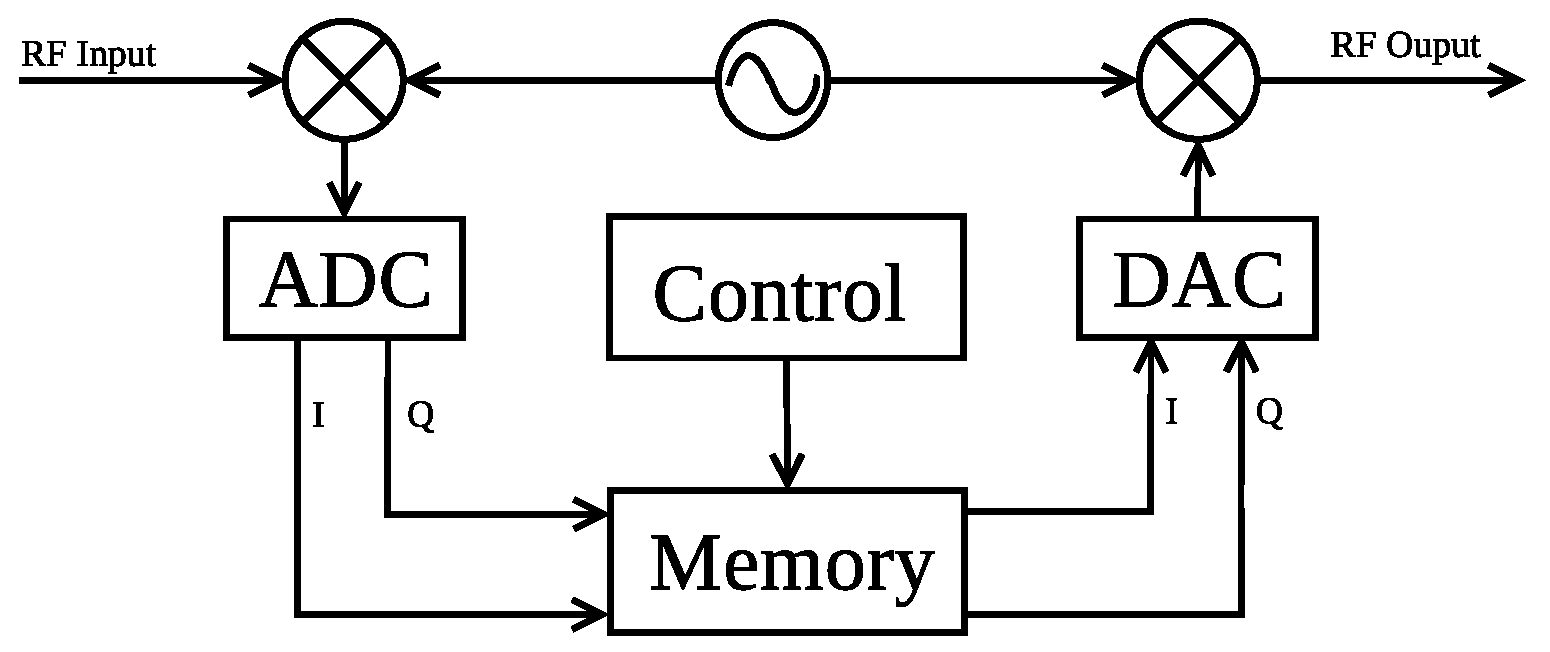
\includegraphics[width=0.8\linewidth]{img/DRFM_Intro}
		\caption{Illustration of DRFM System}
		\label{fig:DRFM_Intro}
	\end{figure}
		



\section{Overview} \label{sec:design}
	\noindent For means of explanation, the architecture of the FPGA based implemented DRFM system can be described by three subsystems. These being, the interfacing and control system, the external peripherals and the DSP system. Whereby each of the constituent systems are monitored and controlled by the top-level controller module. This simplified architecture may be seen in Fig.~\ref{fig:DRFM_Architecture}.\\ \newline This being said, it must be noted that the architecture described in Fig.~\ref{fig:DRFM_Architecture} has not yet been integrated into a RF front end and therefore this paper is a review of the work in progress. The implications of this are that although real time signal processing and data storage are realizable at the speeds dictated by the RF front-end, it has not been shown that this architecture is in fact capable of achieving such speeds.
	\begin{figure*}[h!]
		\centering
		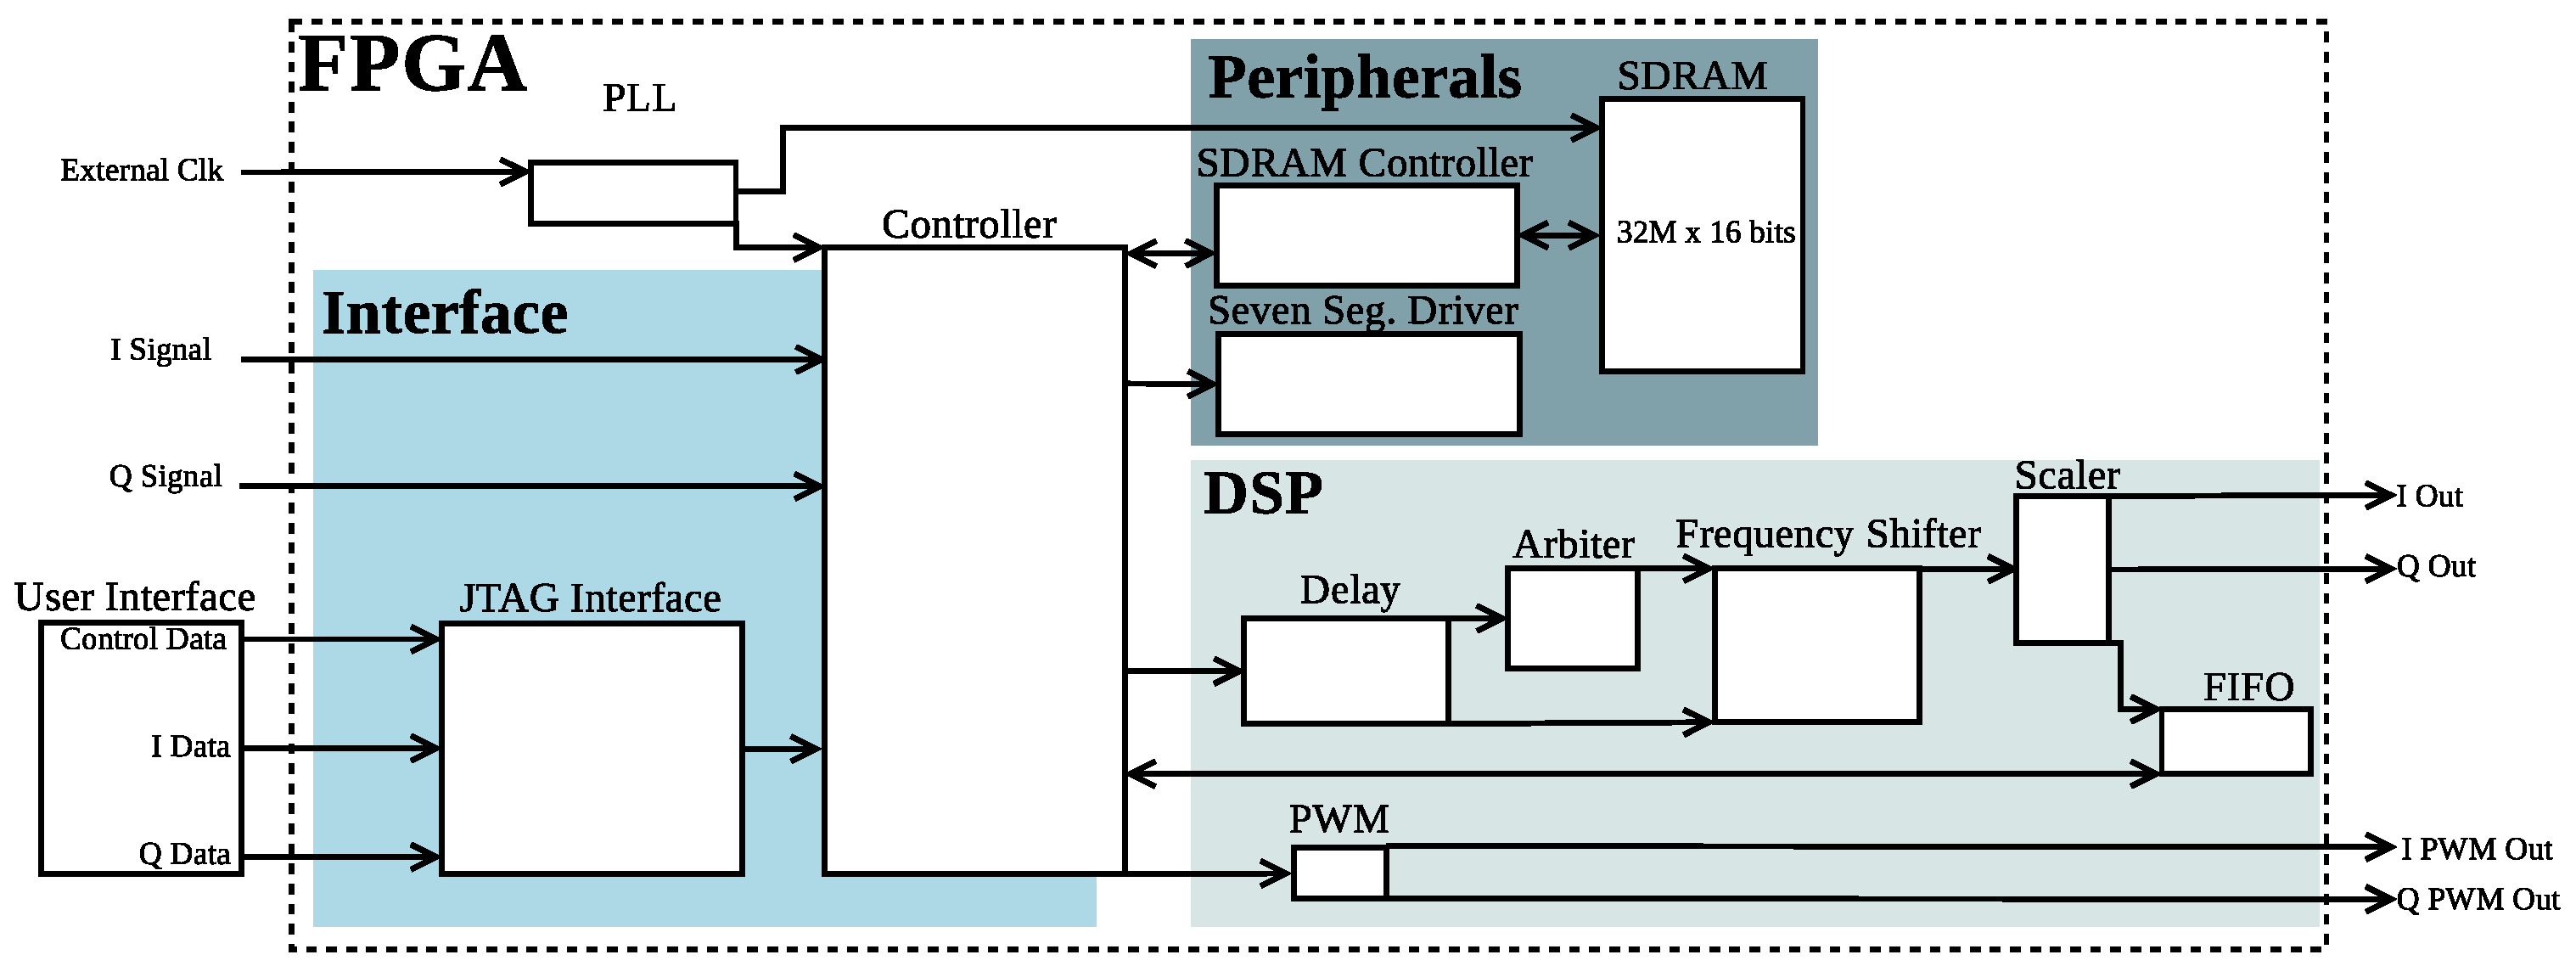
\includegraphics[width=0.95\linewidth]{img/System_Overview}
		\caption{Illustration of the implementation of the  FPGA based DRFM System}
		\label{fig:DRFM_Architecture}
	\end{figure*}
	
	\subsection{JTAG Interface}
		\noindent Joint Action Test Group (JTAG) was originally used as a simplified standard for interconnectivity testing for PCB manufacturing. It was created as a result of Integrated Circuits (IC) pins becoming more densely spaced and therefore classical interconnectivity test approaches were infeasible. The JTAG protocol mitigated the need for physical access to an IC's pins through the use of shift register chains.  \\ \newline In the JTAG standard (IEEE 1149.1) the collections of shift registers are referred to as Boundary Scan Cells (BSCs) which sample and hold data from and to the pin interface. As a result the BSCs can be configured into a serial shift chain thereby allowing to be driving by a serial interface. \\ \newline 	The JTAG interface implemented on the DRFM system allows for software based monitoring, updating and controlling of the DRFM system through the JTAG port.  Through the use of the Altera Virtual JTAG Intellectual Property (IP) core it is possible to access to the JTAG control signals that are routed to the FPGA core, which allow for a fine control over the JTAG resources thereby granting real-time general purpose serial communication \cite{JTAG}. \\ \newline	Through the use of  a Python based User Interface (UI) that runs a TCL JTAG server it is possible to direc
		
	
	\subsection{External Peripherals}
	
	\subsection{Signal Processing}
	
	\subsubsection{Time Delay}
	
	\subsubsection{Frequency shifting}
	
	\subsubsection{Fractional Amplitude Scaling}

	
	




\section{Methodology} \label{sec:implemenation}

\section{Design}
	
	\subsection{System Peripherals}
		\subsubsection{PLL}
		\subsubsection{SDRAM Controller}
		\subsubsection{External SDRAM}
		\subsubsection{PWM}
	
	\subsection{Interface}
		\subsubsection{JTAG Interface}
		\subsubsection{Controller}
		
	\subsection{DRFM Subsystem}
		\subsubsection{Delay}
		\subsubsection{Arbiter}
		\subsubsection{Frequency Shifter}
		\subsubsection{Scaler}

\section{Results} \label{sec:Results}
\noindent Using the implementation described the following results were obtained:
\subsection{Delay}
\noindent Through the use of the Quartus Signal Tap II Logic Analyser \cite{Signal_Tap}, it was possible to probe registers while the implementation was running on the FPGA in real time. As a result screen shots were taken documenting the achievements of the DRFM system. \\ \newline In Fig.~\ref{fig:delay}, the time delay functionality of the system can be seen. The the topmost value of the screen shot, \texttt{rdaddress}, is the address pointer to the RAM delay block. It can be seen that when the value \texttt{time\_delay} changes from 853 to 938 the \texttt{rdaddress} register changes from 1016 to 78 and increments by one for each subsequent clock cycle. It can be also seen that on the cycle after the \texttt{time\_delay} delay line changes, the \texttt{old\_time\_delay} line takes the \texttt{time\_delay}'s value. 
\begin{figure}[h!]
	\centering
	\includegraphics[width=\linewidth]{img/delay}
	\caption{Simulation Output Documenting a Time Delay}
	\label{fig:delay}
\end{figure}

\subsection{Frequency Shift}
	\noindent As already mentioned, the PWM module was used to output the waveforms through a GPIO pin on the FPGA development board. Therefore in order to obtain results about the frequency shift information, an Oscilloscope with FFT functionality was used to measure the frequency information of the PWM outputted signal. The results of the frequency shift were obtained by injecting $y(t)$ into SDRAM which can be expressed mathematically by
		\begin{equation}\footnotesize 
			y = cos(2\pi 10t) + cos(2\pi 20t)  + cos(2\pi 30t) + cos(2\pi 40t)+cos(2\pi 50t). \\
		\end{equation}
	\noindent It can be seen in Fig.~\ref{fig:1khz} that when the frequency shift on the UI was set to 1kHz, the output from the 8 bit PWM had a frequency of 1kHz. Furthermore, when the frequency was changed to 2kHz, the output also changed to 2kHz as can be seen in Fig.~\ref{fig:2khz}.
	\begin{figure}[h!]
	\centering
	\begin{subfigure}{0.48\linewidth}
		\centering
		\includegraphics[width=.9\linewidth]{img/scope_3}
		\caption{Oscilloscope Print of a 1kHz frequency shift }
		\label{fig:1khz}
	\end{subfigure}%
	\begin{subfigure}{0.48\linewidth}
		\centering
		\includegraphics[width=.9\linewidth]{img/scope_4}
		\caption{Oscilloscope Print of a 2kHz frequency shift }
		\label{fig:2khz}
	\end{subfigure}
	\caption{Figures Showing the Measured Frequency Shift}
	\label{fig:2freq}
\end{figure}


\subsection{Amplitude Scaling}
	\noindent By using Quartus Signal Tap II Logic Analyser \cite{Signal_Tap}, it was possible to verify the amplitude scaling functionality of the DRFM system. In Fig.~\ref{fig:full_scale}, a full scale outputted sinusoid can be seen. In Fig.~\ref{fig:attentuated}, a fully attenuated sinusoid can be seen. This is as a result of the user sliding the amplitude scaling slider down to zero.
	\begin{figure}[h!]
	\centering
	\begin{subfigure}[b]{0.55\textwidth}
		\centering
		\includegraphics[width=.9\linewidth]{img/full_scale}
		\caption{Full Scale Sinusoid}
		\label{fig:full_scale}
	\end{subfigure}%


	\begin{subfigure}[b]{0.55\textwidth}
		\centering
		\includegraphics[width=.9\linewidth]{img/attenuated}
		\caption{Fully Attenuated Sinusoid}
		\label{fig:attentuated}
	\end{subfigure}
	\caption{Figures Showing the Measured Amplitude Scaling}
	\label{fig:amp}
\end{figure}

\section{Conclusions}
\noindent From the results, the following conclusions can be drawn.
\subsection{Increased Delay Functionality}
\noindent As shown in the results, the delay function of the DRFM system was clearly working. However, it would be preferable to allow for a longer delay so that the output of the delay could be seen visually when probing with a oscilloscope. This could be achieved by creating a larger RAM block and have a longer delay control word. 
\subsection{Improved Frequency Measurement}
\noindent It can be seen that the output of Fig.~\ref{fig:2freq} is incredibly noisy. This may be attributable to both the fact that the PWM output has some harmonic components and in order to enable a 8 bit output, the 32 bit output vector had to be concatenated. This meant that the concatenation operation, may have resulted in unforeseen harmonic components being captured. \\ \newline This problem could be solved by either performing noise shaping to get a higher resolution PWM output, or by allowing for 2 way JTAG communication so that data could be streamed back to a PC to be analysed more accurately. 

\subsection{Integration into a RF Front-end}
\noindent In order to effectively prove that the DRFM system is functional it should be properly integrated into a RF front-end such as the one shown in Fig.~\ref{fig:DRFM_Intro}. This would allow for the system to be tested more thoroughly, thereby giving a practical measure of its feasibility.

\subsection{Extension to Multiple Targets}
\noindent Finally, a simple way to extend the DRFM system would be to accommodate for multiple targets. This could be a achieved by duplicating the DSP subsystem so that false targets could be synthesized at multiple time delays and frequency shifts. 




%-- Streaming to file.
%-- DAC for sensing.
%-- Noise Shaping for higher resolution output.
%-- multiple targets.
%-- clean up output
\bibliography{References}
\end{sloppypar}
\end{document}

